\documentclass[main.tex]{subfiles}
\begin{document}

\section{Proposed Future Work} % 3pp
\label{sec:future}

Our contributions so far have focussed on developing a compositional and modular model for question answering against text that is capable of performing symbolic reasoning. The ideas presented until now can be extended and improved in innumerable ways. We focus on the following directions for the rest of the thesis.

\subsection{Background on Question Decomposition Meaning Represenation (QDMR)}
Much of our planned future work is based off of the recently proposed resource on Question Decomposition Meaning Represenation~(QDMR;~\newcite{qdmr-2020}) which we explain in this subsection.
This resoures aims at defining a formalism, QDMR, for representing the meaning of questions that is agnostic to any context and is based on \textit{question decomposition}.
QDMR (Figure~\ref{fig:qdmr_examples}) represents complex questions as a sequence of simpler questions that can be executed in that order to answer the original question.
These atomic questions can be thought of as operations performed by a single predicate in a formal semantic parse or a database query (e.g. in SQL or SPARQL).
Unlike semantic parsing though, atomic questions in QDMR are expressed in natural language with the introduction of only a small set of \textit{formal operators}.  Such usage of natural language in the meaning representation allows for representing a much diverse range of questions as compared to lossy logical meaning representation. As expected, the choice of using high-entropy natural language as the basis for meaning representation has its drawbacks.

\begin{figure}[b]
	\centering
    \begin{subfigure}[tb]{0.45\linewidth}
		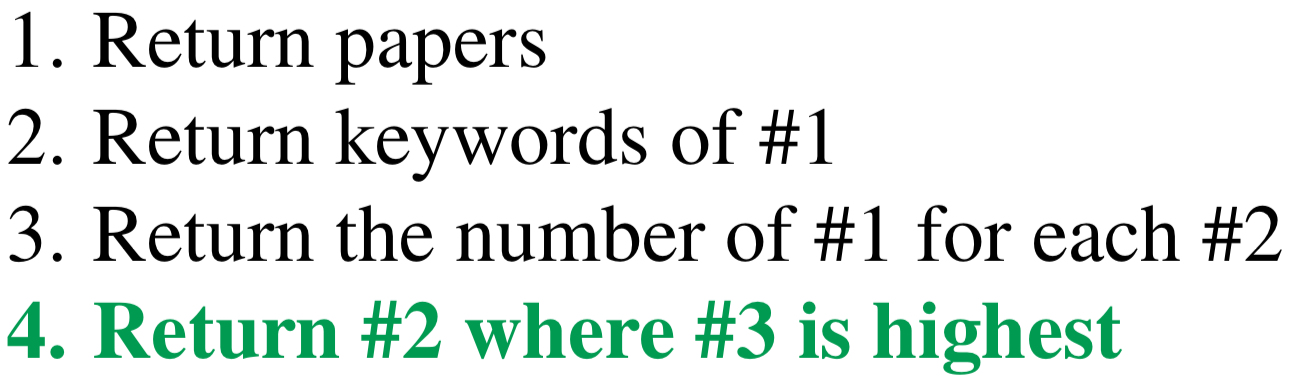
\includegraphics[width=0.8\textwidth]{qdmr_most_example.png}
        \caption{QDMR of \textit{``What is the keyword, which has been contained by the most number of papers?''}}
		\label{fig:qdmr_most}
	\end{subfigure}
    \hfill
    \begin{subfigure}[tb]{0.45\linewidth}
    % \centering
		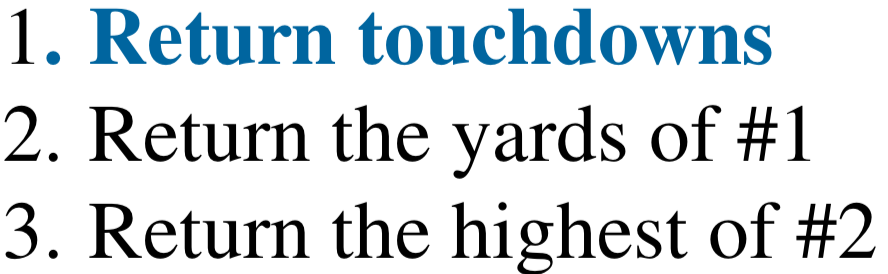
\includegraphics[width=0.65\textwidth]{qdmr_select_example.png}
		\caption{QDMR of \textit{``How many yards was the longest touchdown of the game?''}}
        \label{fig:qdmr_select}
    \end{subfigure}
	\caption{Examples of Question Decomposition Meaning Representation (QDMR)}
	\label{fig:qdmr_examples}
\end{figure}


\subsection{Extending reasoning capabilities}
The reasoning capability of the model we present in Chapter 1 is limited by the kind of modules we define; it cannot answer questions that require semantic operations for which modules do not exist.  % The modules we currently define cannot handle various linguistic constructions, especially those ones that require a symboloc treatment.

\paragraph{Problem}
Our model lacks in modeling various linguistic constructions that would require a symbolic treatment. For example, our model cannot represent determiners such as \textit{``most''} in \textit{``Which player scored the most touchdowns?''} or \textit{``more than half''} in \textit{``Who scored more than half the field goals?''}.
As one extention to our model, we would like to push forward in the direction of trying to design differentiable modules that are capable of handling such generalized quantifiers~\cite{gq-mostowski-1957}.

\paragraph{Potential solution}
Modeling determiners such as \textit{``most''}, \textit{``fewest''}, \textit{``more than 20''} etc. in a differentiable manner is challenging.  It would require us to represent, in a probabilistic manner, the context as sets of elements and properties associated with the elements of the sets, i.e., some kind of a key-value representation.  For example, it would require to represent the unique players who scored touchdown passes (keys) and how many each did (values) in a probabilistic manner.
Such a representation would in turn require one to identify atomic semantic units (e.g. event mentions, entitiy mentions, etc.) from the context which would be needed to identify keys and values.  This is hard to achieve when working with natural language text without any strict and lossy definition of events, entities, etc. and withot supervision of such kind.
% For example, this would require one to, at the least, identify and represent ``events'', ``entities'', and their associated arguments as some discrete units.
Additionally, it would also require identifying equivalence between these semantic units (mentions of entities and events) to cluster mentions of the same concept (for example, to identify unique keys).
The model presented in Chapter 1 made a design choice of having tokens as the basic units of representation which restricts trying to model such quantifiers.  As the next step we are working on having representing module inputs and outputs as logical-sets of text-spans and hope to be able to model more challenging quantifiers with such a represenation.

Since learning a NMN using just question-answer supervision is challenging (Chapter 1), we decide to use QDMR annotations for the DROP dataset as gold question-program supervision which allows to focus on improving program execution and modeling such challenging semantic operators.

\subsection{Transfer learning}
To achieve machine reading in the true sense, we need to develop models in a way such that a single trained model can be applied to answer a diverse set of questions from various domains.  Over the last few years, many reading comprehension datasets have been proposed in various domains (MRQA~\cite{mrqa-2019} provides a representative list) that test for a variety of phenonmenon ranging from simple paraphrase-matching and entity typing to entity tracking and implicative reasoning.
Even then the community largely hasn't focussed on developing a single model that could read and answer questions from various domains, say all the reading comprehension datasets developed until now.  Note that, recently MultiQA~\cite{talmor-multiqa-2019} and submissions to MRQA~\cite{mrqa-2019} did push in this direction but all models were based on fine-tuning a large pretrained language model on multiple datasets.

One key advantage of modular models is the capability to reuse modules in novel contexts, domains, and tasks. We would like to pursue this direction and and as a starting step try to develop a single question answering system that can be trained and evaluated on multiple benchmarks, for example, datasets in Open Reading Benchmark~(ORB;~\newcite{dua-orb-2019}) silmultaneously.  Decomposing the question into multiple atomic questions (via structured programs) would also allow us to study what kind of reasoning primitives can be easily transfered to other domains and which cannot.

\subsection{Systematic Generalization}
% While several machine learning models show extremely good performance on standard iid-test splits, it has been shown that these models often fail to \word{characterize} the underlying linguistic phenomenon and fail to generalize in surprising ways.
There is a growing realization in the NLP community that the traditional supverised learning paradigm, where i.i.d. train/test splits are used to measure model generalization, is not the ideal setup to test NLP models, espcially given the growing size of the models and training datasets that are used.  It has been shown in various studies that models find shortcuts and exploit dataset artifacts to achieve high test-set performance but infact fail in surprising ways on seemingly simple inputs.  Instead, we would like our models to systematically generalize, i.e., actually understand the phenonmena they are trained for and be robust to distributional shifts as long as it results in test instances that are close enough to the training instances.

Though it seems natural that explicitly compositional models should be able to generalize better than black-box models, several works~\cite{sys-generalization-2018,closure-generalization-2020} have shown that it is not necessarily true.  In Chapter 2 we saw that training such compositional models using only end-task supervision does not guarantee that the modules learn to behave in a faithful manner.  Such ill-behaved modules would hamper model's generalization when used in unique configurations.
 We would like to investigate and improve systematic generalization of our model using the recently introduced stress test-sets~\cite{contrast-sets-2020}. Similarly, we are also studying systematic generalization of semantic parsers (extending work from~\newcite{text2sql-2018}) and planning to design parsing models that are mix of Seq2Seq parsers with  parsers that build a logical form over the input~\cite{zettlemoyer-pccg-2005,pasupat-liang-2015,gupta-ncds-2018}.


% King of arbit.


% How do we computationally represent the meaning of language?
% How do we automatically produce these representations from text?

% decisions made a priori about how to represent the world are necessarily lossy

% logical meaning representations

% the structure of the associated program/meaning representation reflects the linguistic structure of question

% formal representations of language

% model structure imitates reasoning and/or linguistic structure

% structured representations of language

% SP has bypassed questions of learning how to represent the world

% can formal (compositional) representations of sentence meaning help us learn reusable operators for perception and reasoning

% What sorts of linguistic phenomena should be explicitly articulated in logical meaning representations, and what distinctions should be left to learning

% automatic discovery of reusable discrete operators for perception and reasoning remains a major challenge -- mike lewis work

% Rather than thinking of question answering as a problem of learning a single function to map from questions and contexts to answers, it’s perhaps useful to think of it as a highly-multitask learning setting, where each problem instance is associated with a novel task, and the identity of that task is expressed only noisily in language

\biblio

\end{document}
